\scanpage{48}\mspage{47}
\uline{Définition} Soient $F,\deleted{F'}G$ deux figures. On dit que $\deleted{F'}G$ est un \uline{raffinement} de $F$, s'il existe une \deleted{\unsure{raffinée|raffinement|raffin}} subdivision $F'$ de $F$, telle que $G\subset F'$ \inserted{sous-figure}.
% slanted
\margin{On écrit $F\ll G$}


On veut que ce soit une relation d'ordre, et pour ceci on va poser

\uline{C 4} Soient $F$ une figure, $G$ une sous-figure \inserted{(i.e. $G$ figure et $G\unsure{\subset|\in}F$)}, $G'$ une subdivision de $G$. Alors \deleted{il existe une subdivision $F'$ de $F$,} \inserted{$G'\cup(F\setminus G)$ est une} subdivision \inserted{de $F$}, et la réunion est disjointe (i.e. \deleted{\unsure{hors|bien}} \inserted{\unsure{de|en} $G$} \margin{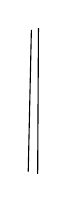
\begin{tikzpicture}[x=1cm,y=1cm]\draw (0,0)--(.04,1.8);\draw (.12,-.03)--(.13,1.82);\end{tikzpicture}}
\[
 \boxed{G'\cap F\subset G}
\]
\deleted{donc} $G'\cap F=G'\cap G$)
% slanted
\margin{C'est \unsure{démenti|démontré} \unsure{par exemple|pour} les strates fermées et str. augmentées\ldots\ \uline{cf plus} bas.}
% slanted
\margin{i.e \unsure{toute} multistrate d'une subdivision de $G$ qui est \uline{compatible} \unsure{avec $F$|sur $G$} \uline{est dans $G$}. OK}
\margin{OK $\nearrow$}
\margin{Corriger : $\exists$ subdivision qui induit $G'$ $+$ la relation $G'\cap\unsure{F^{\to}\subset|F'\subset|F\subset}G$}

\uline{Cor. 1} \uline{Toute} \deleted{raffinement} \inserted{\uline{subdivision}} \uline{d'une sous figure de $F$ est induite par une ``subdivision de $F$}.
\margin{\begin{tikzpicture}\draw (.18,0) .. controls (-.15,.25) and (-.12,.85) .. (.1,1.2);\end{tikzpicture}}

\uline{Cor 2} La relation de raffinement entre figures
\[
 F\ll G
\]
est une relation d'ordre.
% slanted
\margin{OK.}

\deleted{\uline{\unsure{C 5|C 8}} \inserted{\uline{Proposition}} Soient $X,\deleted{\unsure{Y}}\in M$, \inserted{$\deleted{F}G\in\mathcal F$.} Pour que $X\in\deleted{\unsure{F_Y}}G$ \deleted{i.e. $F_X\subset F_Y$} il f. et s. que $X$ et $\deleted{\unsure{Y|F}}G$ compatibles (\unsure{i.e.|comme} $F\equiv F_X\cup\deleted{\unsure{F_Y}}G$ une figure) et $X$ \deleted{raffine} $\inserted{\ll}\deleted{\unsure{F_Y}}G$ i.e $F_X$ raffine $\deleted{\unsure{F_Y}}G$.}
% slanted
\margin{C'est la \deleted{\unsure{Condition|Cons.}} \inserted{définition} de $\leq$ via $\ll$ et $R$}

\deleted{\deleted{\unsure{On}} Supposons en effet que $X$ et $F$ compatibles \deleted{il \unsure{faut|pour} $X\unsure{\text{et}|\phi|,|\in}Y\in F$}, $F$ figure, et que $F_X$ raffine la sous-figure $F_Y= \deleted{\unsure{G.}}$. Donc $\exists$ subd. $G'$ de}
